\chapter{Methods}
\section{Searching Literature}

The PRISMA method \cite{pagePRISMA2020Statement2021}, allows authors to report their findings from a literature search in a clear manner, and was utilised in this dissertation. The PubMed database (\url{https://pubmed.ncbi.nlm.nih.gov/}) houses over 32 million citations and abstracts of biomedical literature. I used PubMed to search for relevant literature relevant to my question: "How effective is deep learning in therapeutic antibody development.". Antibody development is a large area of research, in order to make the research more specific and easier to digest, I broke my research into two segments: Structural prediction of both the antigen and the antibody and then binding prediction between said antigen and antibody.



\subsection{Structural prediction}

\begin{figure}[h!]
    \begin{redbox}{Antibody and antigen structure: Search terms}
        (paratope structure [All Fields] OR ("CDR" [Title] AND "structure" [All Fields]) OR "antibody structure" [All Fields] OR "antibody paratope" [All Fields] OR "antigen-structure" [All Fields] OR "epitope structure" [Title]) AND "deep-learning" [All Fields] 
    \end{redbox}
    \caption{The search terms applied to the PubMed database to identify relevant literature associated with antibody / paratope and antigen / epitope structure.}
    \label{box:antibody_antigen_search}

\end{figure}

To identify literature applying deep learning to antigen and antibody structure I used the search terms shown in \textbf{Figure \ref{box:antibody_antigen_search}} which only produced one result. Whilst deep learning is not a novel technology with the first deep learning network originating in 1965 \cite{ivakhnenkoCYBERNETICPREDICTINGDEVICES1966}. It has only recently gained popularity due to advancements in computing power and learning techniques, reinforcing it as a viable method of computational learning. This is reflected in the lack of literature specific to antibody and antigen structure prediction, a niche topic that is yet to be fully explored. In order to gain a broader set of literature for analysis, I performed a secondary search to find literature associated with protein structure prediction (\textbf{Figure \ref{box:protein_search}}). Antibodies are a form of complex protein, and antigens are very commonly proteins, thus literature on protein structure prediction is applicable to both antibody and antigen structure prediction. I searched with the following search terms:

\begin{figure}[h!]
    
\begin{redbox}{Protein structure: Search terms}
    ('deep-learning'[Title] AND 'protein'[Title] AND 'structure'[Title]) 
    \end{redbox}
    
    \caption{The search terms applied to PubMed to expand literature associated with antibody and antigen structure prediction.}
    \label{box:protein_search}

\end{figure}


These terms produced 22 pieces of literature, totalling 23 results. I excluded any non-primary literature, which includes: reviews, systematic reviews, meta-analysis, and editorials. Then full-text articles were assessed for their eligibility in this dissertation.


\textbf{\subsubsection {Reasons for exclusion}}

Firstly, any literature published prior to 2019 was excluded; rapid developments of computer technologies cause newer deep learning models to rapidly outcompete older programs. This is in tandem with Moore's law \cite{schallerMooreLawPresent1997} which states the number of transistors on integrated circuit boards doubles every year, resulting in a direct increase of processing power. Such advancements of computing power each year on top of novel deep learning techniques, renders older models much less effective and therefore were excluded from the review.
\\[12pt]
Additionally, only literature proposing deep learning programs that aimed to predict structure of the paratope or epitope from the proteins primary amino acid sequence were included. This allows a more accurate representation of how deep learnings could be implemented with other technologies to predict the proteins structure; whilst still modelling the protein structures \emph{ab initio}.
\\[12pt]
After applying my exclusion criteria, there were five relevant papers remaining (\textbf{Figure \ref{fig:PRISM-structure}}).

\begin{figure}[H]
    \centering
    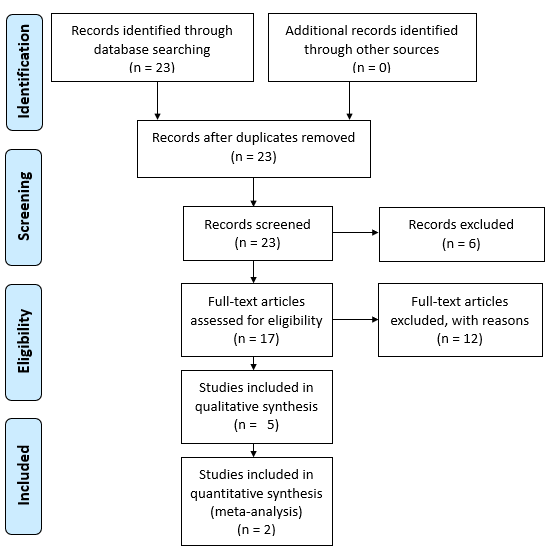
\includegraphics[width=0.6\linewidth]{./images/flow_diagram_structures.png}
    \caption{\textbf{PRISMA flow diagram} selection process for antibody + antigen structure literature. Searches used (\textbf{Figure \ref{box:protein_search}}) and (\textbf{Figure \ref{box:antibody_antigen_search}})}
    \label{fig:PRISM-structure}
\end{figure}

\subsection{Antibody-Antigen binding predictions}

\begin{figure}[H]
    \begin{redbox}{Protein-Protein interaction: Search terms}
        (antibody-antigen[Title] OR paratope-epitope[Title] or protein-protein-interactions or PPI) AND (deep learning) 
    \end{redbox}
    \caption{The search terms applied to PubMed to expand literature associated with antibody and antigen binding prediction.}
    \label{box:ppi_search}

\end{figure}

I began my search trying to identify models that predict antibody-antigen binding from their primary sequence, but I was unsuccessful. Again this is probably due to a lack of research specific to antibody-antigen interaction prediction. Fortunately, general protein-protein interactions have been researched a fair amount; and as antibody-antigen interactions often represent protein protein interactions, research into this area would be suitable to evaluate deep learnings ability in predicting antibody-antigen binding. My search terms produced 81 results \textbf{Figure \ref{box:ppi_search}}. Once I had excluded any non-primary literature as seen previously, there were 62 articles ready to be reviewed for eligibility (\textbf{Figure \ref{fig:PRISM-interactions}}).

\begin{figure}[H]
    \centering
    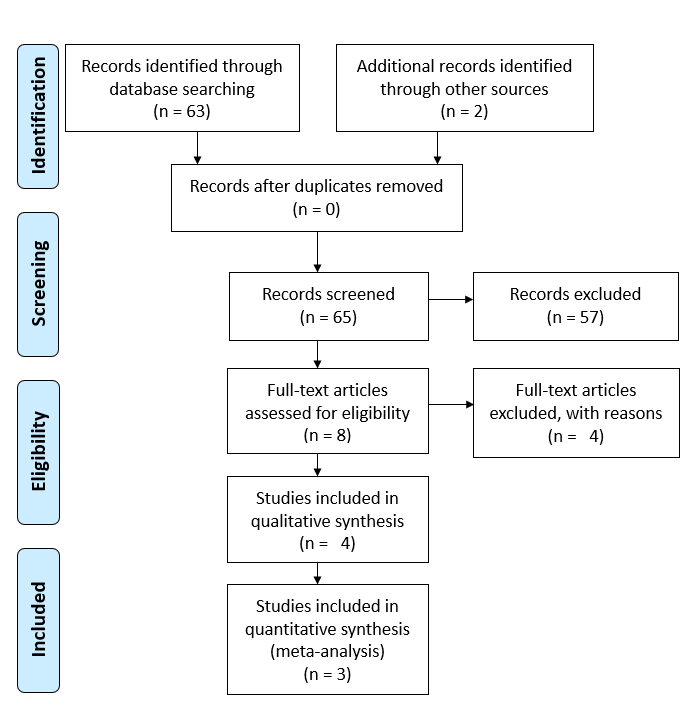
\includegraphics[width=0.6\linewidth]{./images/flow_diagram_interactions.png}
    \caption{\textbf{PRISMA flow diagram} selection process for antibody-antigen interaction literature.}
    \label{fig:PRISM-interactions}
\end{figure}

I excluded any papers prior to 2018 and papers that did not predict binding interactions via contact prediction were excluded. Additionally, papers associated with MHC and TCR binding are not relevant to the binding interactions of antibodies, thus these papers were also excluded.
\\[12pt]
The literature selected for analysis is shown in (\textbf{Figure \ref{tab:literature-overview}}).

\begin{table}[H]
    \begin{small}
        \caption{Deep learning programs from papers discovered in the literature search.}
        \label{tab:literature-overview}
        \begin{center}
            \begin{tabular}[c]{l|l}
                \hline
                \multicolumn{1}{c|}{\textbf{Structure Prediction}} & 
                \multicolumn{1}{c}{\textbf{Interaction Prediction}} \\
                \hline
                AlphaFold \cite{seniorImprovedProteinStructure2020} & DeepInterface \cite{balciDeepInterfaceProteinproteinInterface2019} \\
        
                DeepH3 \cite{ruffoloGeometricPotentialsDeep2020}  & DNN-PPI \cite{liDeepNeuralNetwork2018}  \\
                DeepAccNet \cite{hiranumaImprovedProteinStructure2021} & DPPI \cite{hashemifarPredictingProteinProtein2018} \\
                MULTICOM \cite{houMULTICOMProteinStructure2020a} &  ParaPred \cite{liberisParapredAntibodyParatope2018} \\
                RaptorX \cite{xuAnalysisDistancebasedProtein2019} & PINet \cite{daiProteinInteractionInterface2021} \\
                
                \hline
            \end{tabular}
        \end{center}
    \end{small}
\end{table}


\subsection{CASP13 comparison}

I extracted global distance test total scores (GDT\_TS) and GDT high accuracy scores (GDT\_HA) from CASP13's official website \href{https://predictioncenter.org/casp13/}{predictioncenter.org/casp13}, for groups 43 (AlphaFold), 89 (MULTICOM), and 324 (RaptorX). I separated the results with the following categories: template based modelling, free modelling, and contact prediction. I performed a one-way anova to test if any of the models performed significantly better than their counterparts for all three categories.

\subsection{Testing for an overfit}
To test for an overfit of the ParaPred model \cite{liberisParapredAntibodyParatope2018} I curated a test set of antibody-antigen structures, 3 from within the ParaPred training set, and 3 from the SAbDab \cite{dunbarSAbDabStructuralAntibody2014} that were not in the ParaPred training set. The combined dataset totalled 476 residues from 36 CDRs. I entered the primary sequences of these antibodies to the ParaPred program, which extracted CDR sequences using the Cothia numbering scheme \cite{al-lazikaniStandardConformationsCanonical1997} and that produced a list of outputs between 1 and 0 for each residue representing bound or unbound from the antigen respectively (\textbf{Figure \ref{fig:ParaPredOutput}}). 

\begin{figure}[H]
    \begin{small}
        \begin{center}
            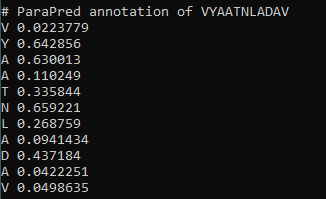
\includegraphics[width=0.5\textwidth]{./images/parapred_output.png}
        \end{center}
        \caption{\textbf{Example output from the ParaPred program \cite{liberisParapredAntibodyParatope2018}}. Each value represents a binding prediction between 1 and 0 for the associated residue to its left.}
        \label{fig:ParaPredOutput}
    \end{small}
\end{figure}

ParaPreds curators treated residues as bound if an atom belonging to a residue is within 4.5Å of any part of the antigen\cite{liberisParapredAntibodyParatope2018}. To confirm which residues I should treat as bound for comparison to the ParaPred output, I used python and a library called BioPython \cite{cockBiopythonFreelyAvailable2009}, my code is available here: \href{https://github.com/mah51/determine-bound-residues}{https://github.com/mah51/determine-bound-residues}. I calculated the absolute error between the predicted value outputted from ParaPred and the actual bound value determined by my program, for each residue. I performed a Welch t-test using this absolute error to determine if the difference in means between the structures from within ParaPred's training set and those that were not, was significant.


